% !TeX TXS-program:compile = txs:///pdflatex/[--shell-escape]
\documentclass[10pt,landscape,a4paper]{article}
\usepackage[table]{xcolor}
\usepackage[normalem]{ulem}
\usepackage{tikz}
\usetikzlibrary{shapes,positioning,arrows,fit,calc,graphs,graphs.standard}
\usepackage[nosf]{kpfonts}
\usepackage[t1]{sourcesanspro}
\usepackage{multicol}
\usepackage{wrapfig}
\usepackage[top=0mm,bottom=0mm,left=1mm,right=1mm]{geometry}
\usepackage[framemethod=tikz]{mdframed}
\usepackage{microtype}
\usepackage{tabularx}
\usepackage{graphicx}
\usepackage{hhline}
\usepackage{makecell}
\usepackage{mathtools}
\usepackage{subfig}
\usepackage{listings}
\usepackage{soul}
\usepackage{amsmath,amsthm,amsfonts,amssymb}
\usepackage{wrapfig}
\usepackage{booktabs}

\graphicspath{ {./img/} }

\DeclarePairedDelimiter{\ceil}{\lceil}{\rceil}

\newcommand\codeblue[1]{\textcolor{blue}{\code{#1}}}

\definecolor{myblue}{cmyk}{1,.72,0,.38}

\pgfdeclarelayer{background}
\pgfsetlayers{background,main}

\renewcommand{\baselinestretch}{.8}
\pagestyle{empty}

\let\counterwithout\relax
\let\counterwithin\relax
\usepackage{chngcntr}
\usepackage{verbatim}
\usepackage{etoolbox}
\makeatletter
\preto{\@verbatim}{\topsep=0pt \partopsep=0pt }
\makeatother

\counterwithin*{equation}{section}
\counterwithin*{equation}{subsection}
\usepackage{enumitem}
\newlist{legal}{enumerate}{10}
\setlist[legal]{label*=\arabic*.,leftmargin=3mm}
\setlist[itemize]{leftmargin=2.5mm}
\setlist[enumerate]{leftmargin=3mm}
\setlist{nosep}
\usepackage{minted}
\def\code#1{\texttt{#1}}
\makeatletter

\renewcommand{\section}{\@startsection{section}{1}{0mm}%
	{.2ex}%
	{.2ex}%x
	{\color{myblue}\sffamily\scriptsize\bfseries}}
\renewcommand{\subsection}{\@startsection{subsection}{1}{0mm}%
	{.2ex}%
	{.2ex}%x
	{\sffamily\bfseries}}
\renewcommand{\subsubsection}{\@startsection{subsubsection}{1}{0mm}%
	{.2ex}%
	{.2ex}%x
	{\rmfamily\bfseries}}

\makeatother
\setlength{\parindent}{0pt}
\setminted{tabsize=2, breaklines}
% Remove belowskip of minted
\setlength\partopsep{-\topsep}

\newcolumntype{a}{>{\hsize=1.5\hsize}X}
\newcolumntype{b}{>{\hsize=.25\hsize}X}

\setlength\columnsep{10pt}
\setlength\columnseprule{0pt}
\begin{document}
	\tiny
	\begin{multicols*}{4}
		\raggedcolumns
		\section{Software Development Process}
%		\subsection{Origins of SE}
%		\begin{itemize}
%			\item In 1963-1964, Margret Hamilton, lead developer for Skylab and Apollo program, coined the term \textit{software engineering}
%			\item Used again in 1968/69 by Bauer at NATO software engineering conference in response to software crisis in th 1960s
%			\begin{itemize}
%				\item mainly concerned with time, cost and quality of software developed
%				\item researched and developed Software development process models, architectures, design principles, testing methods and design patters
%			\end{itemize}
%			\item 2nd round of software crisis in the 1970s
%			\begin{itemize}
%				\item 'push' factors such as advances in hardware, reductions in hardware costs, increase in processing power, device proliferation, large amount of data available
%				\item 'pull' factors such as have higher demand due to influx of digital natives
%				\item researched and developed on data analytics, security, cloud computing, edge computing, DevOps (CI/CD), microservices
%			\end{itemize}
%		\end{itemize}
		\subsection{Types of Software Applications}
		\begin{enumerate}         
			\item \textbf{Embedded} - An embedded system is a microprocessor-based computer hardware system with software that is designed to perform a dedicated function, either as an independent system or as a part of a large system e.g. Cameras, MP3, Calculators
			\item \textbf{Real-Time} - “real-time system” refers to any information processing system with hardware and software components that perform real-time application functions and can respond to events within predictable and specific time constraints e.g. video conferencing, online gaming
			\item \textbf{Concurrent} - Concurrent systems are systems comprising a collection of independent components which may perform operations concurrently e.g. web servers that service many different connections
			\item \textbf{Distributed} - computing environment in which various components are spread across multiple computers e.g. Telephone and cellular networks
			\item \textbf{Open content systems} - Source code not released to public but content is publicly available e.g. Wikipedia, FaceBook, YouTube, Twitter, Flickr
			\item \textbf{Open Source System} - Source code is openly available e.g. Linux, Apache
		\end{enumerate}
		\subsection{Variations}
		\begin{itemize}
			\item \textbf{Requirements}: Known vs Emerge from crowd
			\item \textbf{Process}: Planned increment vs No stable state/version
			\item \textbf{Resources}: Dedicated and managed vs Adhoc resources
			\item \textbf{Contributors}: Controlled vs influenced
		\end{itemize}
		\subsection{Edge Computing}
		\begin{itemize}
			\item Edge computing is a distributed computing paradigm that \textbf{brings computation and data storage closer to the sources of data} e.g. IoT devices
			\item Balance the demands of centralized computing and localized decision-making
		\end{itemize}
		\subsubsection{Decentralized vs Centralized Computing}
		\begin{itemize}
			\item \textbf{Decentralized Computing} - Everyone has a computer, everyone is computing something
			\item \textbf{Centralized Computing} - Type of computing architecture where most/all of the processing is down on a central server e.g. SoC Compute Cluster, IBM Mainframe
			\item Cloud computing is a mixture of decentralized and centralized computing
		\end{itemize}
		\subsubsection{Motivation for Edge Computing}
		\begin{itemize}
			\item Cloud-based applications have a \textbf{significant amount of latency} as there is a time delay between request and response from server
			\item For many critical tasks that \textbf{need immediate computation} for e.g. Tesla's auto driving system, we cannot afford the latency and hence computation must be done at edge
		\end{itemize}
		\subsubsection{Limitations of Edge Computing}
		\begin{itemize}
			\item \textbf{Limited computation power} in edge computers
			\item Many of devices at edge are not connected to a power source $\rightarrow$ \textbf{issues of battery life and heat dissipation}
			\item Typical solution to these problems is to combine the power of cloud and edge computing together
		\end{itemize}
		\subsection{Software Development}
		\subsubsection{Factors affecting Software Development}
		\begin{itemize}
			\item \textbf{Requirements} - known at the start? determines complexity of software
			\item \textbf{Process} - Waterfall? Agile? What resources and time is needed for the process?
			\item  \textbf{Criticality} - Strict deadline? Experimental? What are the consequences of failure?
			\item \textbf{People/Resources} - What resources are available? What are the competence of the engineers? What technologies are available?
		\end{itemize}
		\subsubsection{Process Models}
		Waterfall, Spiral, Rapid Programming, eXtreme Programming, Rational Unified Process (RUP), Test Driven Development, Agile (Scrum, Crystal etc.)
		\subsubsection{Agile Process}
		\begin{minipage}{0.55\columnwidth}
			\begin{center}
				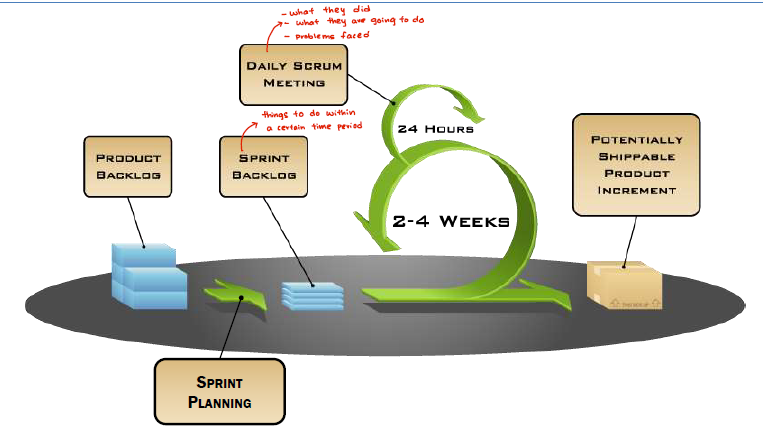
\includegraphics[width=1\columnwidth]{agile_lifecycle}
			\end{center}
		\end{minipage}
		\begin{minipage}{0.45\columnwidth}
			\begin{itemize}
				\item Agile is a \textbf{methodology/ideology} that emphasizes iterative development and cross-functional collaboration
%				\item Individuals and interactions over processes and tools
%				\item Working software over comprehensive documentation
%				(fastidious paperwork, not dev docs)
%				\item Customer collaboration over contract negotiation
%				\item Responding to change over following a plan
				\item Done using \textbf{SCRUM}.
				\begin{itemize}
					\item Work is done in sprints, where a subset of the product backlog is cleared
					\item Project Backlog is a piece of document noting down the FRs, along with their priority and the sprint to be completed in, typically \textbf{done after user stories}
					\item Often have a 15 min scrum meeting at the start of the day to discuss what is done, what is in progress and what is to be done
				\end{itemize}
			\end{itemize}
		\end{minipage}
		\subsection{Software Delivery}
		\begin{itemize}
			\item \textbf{Deployment pipeline}: an automated implementation of application build, deploy, test, and release process
			\item Typical development pipeline: Dev $\rightarrow$ Test $\rightarrow$ User acceptance $\rightarrow$ Production
		\end{itemize}
		\subsubsection{CI/CD Pipeline}
		\begin{itemize}
			\item \textbf{Continuous Integration} - development practice that requires developers to integrate code into a shared repository several times a day. Each check-in is	then verified by an automated build (typically in a staging env that is very similar to production env), allowing teams to detect problems early
			\item \textbf{Continuous Delivery} - ensuring that every good build is potentially
			ready for production release, \textcolor{red}{manual deployment to production}
			\item \textbf{Continuous Deployment} - \textcolor{red}{automating the release} of a good build
			to the production environment
		\end{itemize}
%		\begin{center}
%			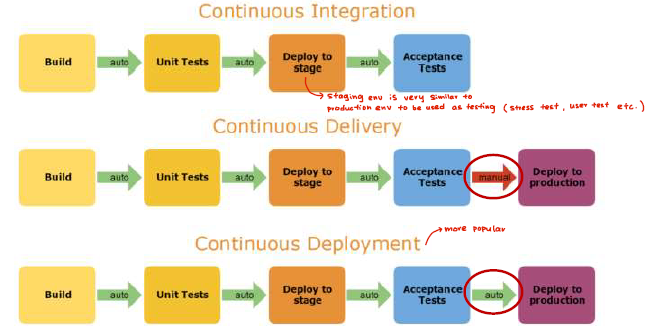
\includegraphics[width=0.55\columnwidth]{ci_cd}
%		\end{center}
		\subsubsection{DevOps}
		\begin{itemize}
			\item DevOps is a set of \textbf{software development practices/process} that combine software development (Dev) and operations (Ops)
			\item intends to reduce the	time between committing a change to a system and the change being placed into normal production while ensuring high quality
			\item It is the intersection of Dev, QA and Technology Ops
		\end{itemize}
		\underline{DevOps Pipeline}
		\begin{itemize}
			\item Push code $\rightarrow$ Pull code and build $\rightarrow$ Test $\rightarrow$ Store artifacts and build repo $\rightarrow$ Deploy and release $\rightarrow$ Config Env $\rightarrow$ Update DB $\rightarrow$ Update apps $\rightarrow$ Push to users$\rightarrow$ App and Network Performance monitoring
		\end{itemize}
%		\begin{center}
%			
\includegraphics[width=0.7\columnwidth]{devops_pipeline}
%		\end{center}
		\underline{DevOps Benefits}
		\begin{itemize}
			\item Uses CI/CD, Continuous Monitoring/Logging, Communication and collaboration and IaaS (e.g. GitHub Actions) to achieve the following benefits:
		\end{itemize}
		\begin{center}
			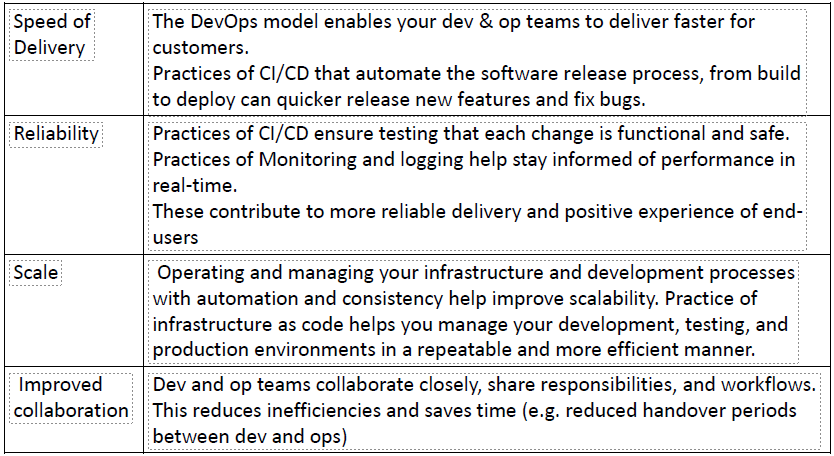
\includegraphics[width=0.64\columnwidth]{devops_benefits}
		\end{center}
%		\subsection{Summary}
%		\begin{itemize}
%			\item Software is a system of intercommunicating (software)
%			components
%			\item Designing a system requires a systematic and rigorous approach
%			demanded by the scale and complexity of the requirements
%			\item Software development is a set of tasks to design and implement
%			requirements for a software system. \\
%			The artifacts – code, models, and documents, represent the solution.
%		\end{itemize}
		\section{Specifying Software Requirements}
		\subsection{What is a Requirement}
		\begin{itemize}
			\item condition or \textbf{capability needed by a user} to solve a
			problem or achieve an objective
			\item \textbf{capability that must be met or possessed by a
			system}
			\item \textbf{Specification} of what should be implemented
			\item Can be thought of as a contract of how a system should behave (functionalities)
		\end{itemize}
		\subsubsection{Examples of Requirements}
		\begin{itemize}
			\item \textbf{User stories} 
			\begin{itemize}
				\item \textcolor{red}{User centric}
				\item Format:  "As a \{role\} I want to \{functionality\} so that I \{what is achieved\}"
				\item Could include constraints to bound the requirement even tighter (\textbf{NFRs})
			\end{itemize}
			\item \textbf{Non-user story format}
			\begin{itemize}
				\item \textcolor{red}{Product centric}
				\item Danger of giving users functionality that they did not request for, need to ensure that it is in sync with what users want
				\item Typically have a better or more refined description
				\item e.g. The system will support the following file formats: png, jpeg, bmp, tiff
				and gif
			\end{itemize}
			\item Class Responsibilities Collaborator (CRC) Model
			\begin{itemize}
				\item Follows OOP
				\item Uses a collection of stand index cards divided into 3 sections
				\item \textbf{Class}: represents collection of similar objects
				\item \textbf{Responsibility}: something the class knows/does
				\item \textbf{Collaborator}: another class that a class
				interacts with to fulfill its responsibilities
			\end{itemize}
			\item Specifying Microservices Requirement
			\begin{itemize}
				\item Typically in a table format with Name of MS, Description, Capabilities, Service API (Async, sync calls, commands, events published), NFRs
				\item Should contain Consumer Tasks, Interface, Qualities, Logic/Rules, Data, Dependencies
			\end{itemize}
		\end{itemize}
		\subsubsection{Types of Requirements}
		\begin{itemize}
			\item \textbf{Business Requirements}: Why the organization is implementing the system (recorded in vision and scope), e.g. reduce staff costs by 25\%
			\item \textbf{User Requirements}: Goals the user must be able to perform with the product, e.g. check for a flight using the website
			\item \textbf{System Requirements}: Hardware or software issues, e.g. the invoice system must share data with the purchase order	system. Affects functional requirements
			\item \textbf{Quality Attributes/NFR}: How well the system performs, e.g. mean time between failure $\geq$ 100 hours. A type of non-functional requirement (code could be involved)
			\item \textbf{Functional Requirements}: The behavior the product will exhibit, describes what developers must implement, e.g. passenger shall be able to print boarding passes.
			\item \textbf{Constraints}: Limitations on design and implementation choices, e.g. must be backwards compatible. A type of non-functional requirements
			\item \textbf{Data Requirements}: Describes data items or structures, e.g. product number is alphanumeric
			\item \textbf{Business Rules}: Policies/regulations/guidelines/standards. Constraints business, user and functional requirements e.g. staff gets 30\% off
			\item \textbf{External Interfaces}: Describes connections between your system and outside world, e.g., must import files in CSV format
			\begin{center}
				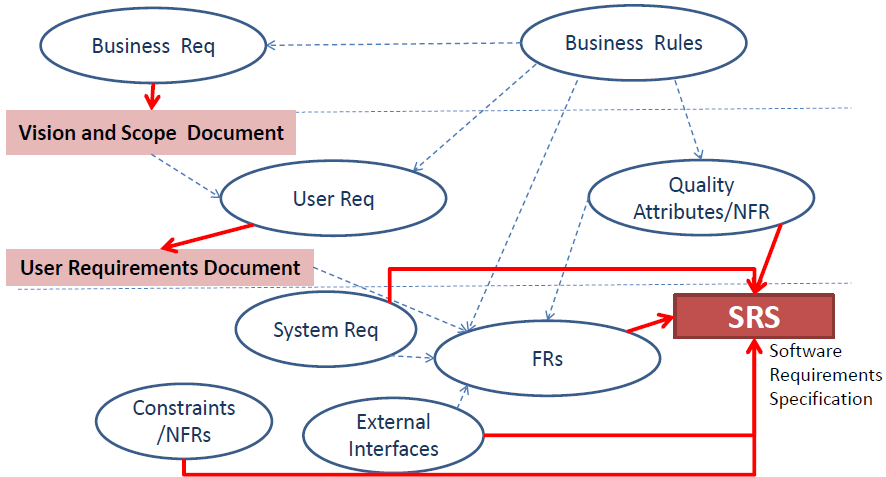
\includegraphics[width=0.5\columnwidth]{reqs}
			\end{center}
		\end{itemize}
		\subsection{User (URS) vs Software (SRS) Requirement Specification}
		\begin{itemize}
			\item User requirement describes the \textbf{end-user requirements} for a system
			\item Software requirements describes \textbf{what the system must do}
			\item \textcolor{red}{SRS could include URS but URS will not include SRS}
			\item SRS needs to be accurate, complete, consistent, testable, modifiable, ranked, traceable, verifiable and valid
			\item URS audience - End-users, SRS audience - Developers, specification of Acceptance Testing
		\end{itemize}
%		\subsection{Requirements Development Phase}
%		\begin{enumerate}         
%			\item \textbf{Elicitation}: Discover requirements through interviews, workshops, document analysis or prototyping
%			\item \textbf{Analysis}: Analyze, decompose, derive, understand, negotiate requirements, identify gaps
%			\item \textbf{Specification}: written and illustrated requirements for comprehension, review and use
%			\item \textbf{Validation}: Confirm correct set of requirements that will enable developers to build a solution
%		\end{enumerate}
%		\begin{center}
%			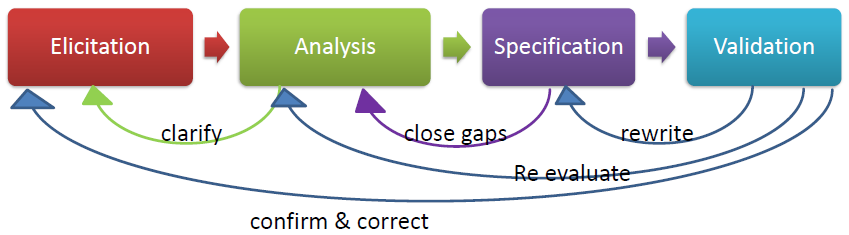
\includegraphics[width=0.5\columnwidth]{req_dev_proc}
%		\end{center}
		\subsection{Sources of Software Requirements}
		\begin{itemize}
			\item Note that all e.g. below are user-centric
		\end{itemize}
		\begin{center}
			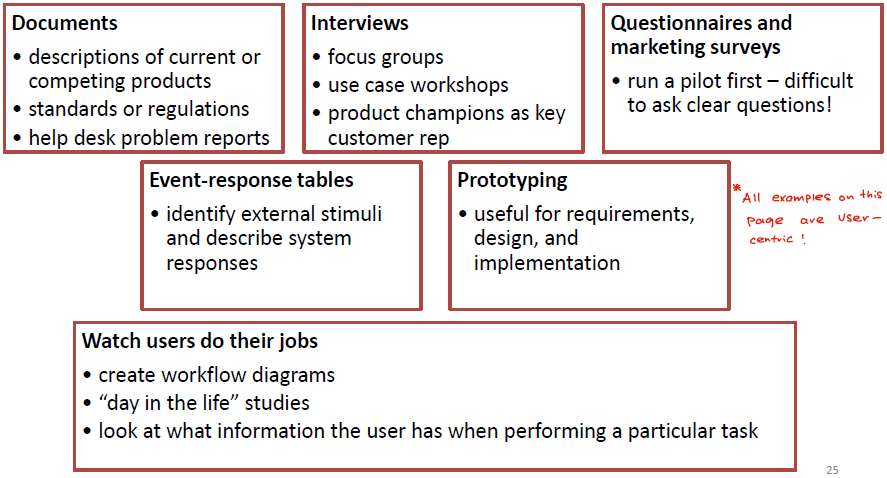
\includegraphics[width=0.5\columnwidth]{req_sources}
		\end{center}
%		\subsection{Software Requirement Specification}
%		\subsubsection{SRS Components}
%		Notice that most of the components are NFRs/Quality Attributes
%		\begin{itemize}
%			\item Interfaces
%			\item Functional Capabilities
%			\item Performance Levels
%			\item Data structure/Elements
%			\item Safety
%			\item Reliability
%			\item Security/Privacy
%			\item Quality
%			\item Constraints and limitations
%		\end{itemize}
%		\subsubsection{Qualities of a good SRS}
%		\begin{itemize}
%			\item Accurate
%			\item Complete and consistent
%			\item Modifiable
%			\item Ranked
%			\item Testable
%			\item Traceable
%			\item Unambiguous
%			\item Verifiable
%			\item Valid
%		\end{itemize}
		\subsection{Quality Attributes}
		\subsubsection{External Quality Attributes}
		\begin{itemize}
			\item \textbf{Availability}: Measure of the planned up time during which the system is fully operational
			\item \textbf{Installability}: How easy it is to install the system for the end-user
			\item \textbf{Integrity}: Preventing information loss and preserving data correctness
			\item \textbf{Interoperability}: How readily the system can exchange data and services with other software and hardware
			\item \textbf{Performance}: Responsiveness to user actions. May also compromise safety if e.g. a safety system responds poorly
			\item \textbf{Reliability}: Probability of software executing without failure for a specific period of time
			\item \textbf{Robustness}: Degree to which a system performs when faced with invalid inputs, defects and attacks
			\item \textbf{Safety}: Prevents injury or damage to people or property
			\item \textbf{Security}: Authorisation, authentication, confidentiality, etc
%			\begin{itemize}
%				\item Traditionally, security is considered during the \textbf{design phase} of Software Development
%				\item However, if we do not consider it during SRS stage, it is likely that some security requirements will be overlooked
%				\item Specifying security features at the SRS ensures that Acceptance
%				Tests include testing for those security features $\rightarrow$ significantly improves security assurance of software
%				\item Would want business owners to decide on security requirements as they are best positioned to decide tradeoffs
%				\item Typical security requirements: how to resolve forgotten passwords, account lockouts, inactive sessions, what activities are logged and what level of detail is the logging, what activity considered suspicious
%			\end{itemize}
			\item \textbf{Usability}: User-friendliness and ease of use
		\end{itemize}
		\subsubsection{Internal Quality Attributes}
		\begin{itemize}
			\item \textbf{Efficiency}: How well the system utilises the hardware, network etc
			\item \textbf{Modifiability}: How easily designs and code can be understood, changed and extended
			\item \textbf{Portability}: Effort needed to migrate the software from one environment to another
			\item \textbf{Reusability}: Effort required to convert a software component for use in other apps
			\item \textbf{Scalability}: Ability to grow to accommodate more users, servers, locations, etc. without compromising performance or correctness
			\item \textbf{Verifiability}: How well the software (components) can be evaluated to demonstrate that it functions as expected
		\end{itemize}
		\subsubsection{Quality Attributes Requirements of Different Systems}
		\begin{itemize}
			\item Embedded software: performance, efficiency, reliability, robustness, safety, security
			\item Internet Application: availability, integrity, interoperability, performance, scalability, security, usability
			\item Desktop/Mobile software: performance, security usability
		\end{itemize}
%		\begin{center}
%			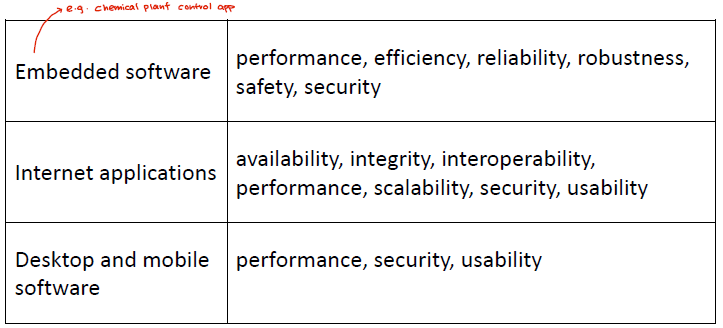
\includegraphics[width=0.5\columnwidth]{quality_attribute_requirement}
%		\end{center}
		\subsubsection{Quality Attribute Tradeoffs}
		\begin{tabular}{c c}
			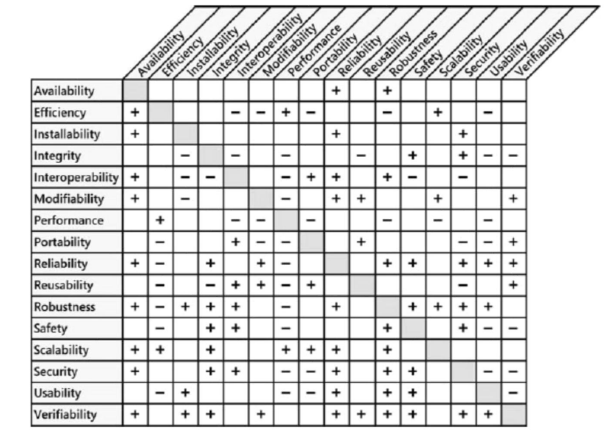
\includegraphics[width=0.49\linewidth]{qa_tradeoff}
			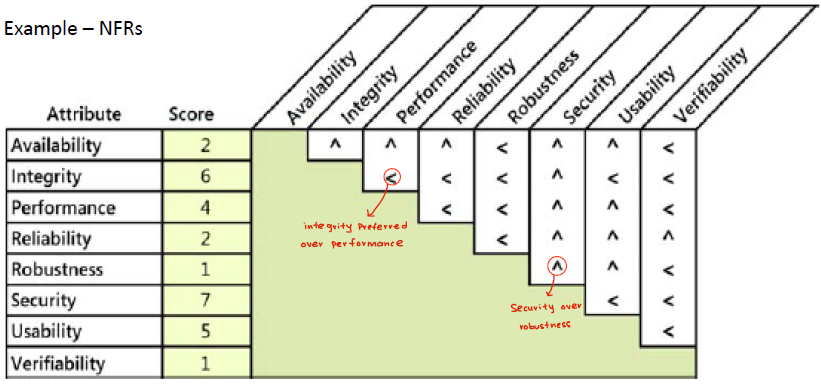
\includegraphics[width=0.51\linewidth]{req-prio}
		\end{tabular}
%		\subsubsection{Prioritization Technique}
%		\begin{itemize}
%			\item High-Med-Low
%			\item Must-Should-Could-Wish
%			\item \$100 approach
%			\item Quality-Function-Deployment
%		\end{itemize}
		\subsubsection{Safety vs Security}
		\begin{itemize}
			\item \textbf{Safety}: About whether a system can harm someone or something physically, financially, reputation etc. e.g. User should be able to see list of options with ingredients highlighted in red that are known to cause allergic reaction
			\item \textbf{Security}: about privacy, auth and integrity. e.g. Is data protected from disclosure, is system only accessible to authorized users.
			\begin{itemize}
				\item Security breaches \textbf{typically involve some sort of financial harm}
			\end{itemize}
		\end{itemize}
		\subsubsection{Validation vs Verification}
		Validation is about whether you have the \textbf{right requirements} and if they \textbf{trace back to the business objectives}. Verification is whether you have written the requirements right i.e. complete, correct, feasible, priority unambiguous. Can be checked informally by passing the requirements around or formally through formal inspection 
%		\subsection{Forms of Documentations}
%		\begin{itemize}
%			\item Textual
%			\begin{itemize}
%				\item Vision and Scope Document
%				\item Use case Document
%				\item SRS
%			\end{itemize}
%			\item Visual
%			\begin{itemize}
%				\item Structured analysis models: Data flow diagram, entity-relationship diagram, state-transition diagram, dialog map, Object-oriented analysis models
%			\end{itemize}
%		\end{itemize}
		\section{Software Architectures}
		Software Architecture design represents the structure and relationship of data and program components that are required to build a software. It helps to form some sort of \textbf{pattern} which allows certain type of application to reuse these architectures e.g. MVC. Building blocks of software architecture includes:
		\begin{itemize}
			\item \textbf{Component}: models an application-specific
			function
			\item \textbf{Connector}: models Interactions	among components for the purpose of transfer of control and/or data
			\item \textbf{Configuration}: Topology or structure
		\end{itemize}
		\subsection{Basic Concepts \& Definitions}
		\begin{itemize}
			\item Control Flow
			\begin{itemize}
				\item Computation order
				\item An arrow from 1 block in architecture diagram to another block typically means that there is some sort of sequence where the latter is performed after the formal block
				\item How the focus of control moves throughout the execution. Data may accompany control. e.g. in a CI pipeline, control is passed when it moves from \texttt{Build}  to \texttt{Test}
			\end{itemize}
			\item Data Flow
			\begin{itemize}
				\item data availability, transformation, latency
				\item How data moves through a collection of computations
				\item As data moves, control is activated $\rightarrow$ Data and Control flows are interlinked
			\end{itemize}
		\end{itemize}
		\subsection{Call and Return}
		\begin{enumerate}
			\item \textbf{Hierarchical} (synchronous)
			\begin{itemize}
				\item control moves from one component to another and back
				\item consists of main program and procedures (possibly also sub-procedures)
				\item "use" relation between components $\rightarrow$ arrow direction indicates which components calls what other component
				\item \textbf{Single thread of control}
				\item \textbf{Hierarchical decomposition}: correctness of a procedure depends on
				correctness of its sub-procedures
			\end{itemize}
			\item \textbf{Non-hierarchical}
			\begin{itemize}
				\item Components communicate via Event notifications / Message passing / RPC and other protocols (could be async / sync, P2P or published)
				\item No strict hierarchy between components
			\end{itemize}
		\end{enumerate}
		\begin{itemize}
			\item \textbf{Pros}: Easy to modify, easy to extend by adding modules, easy to analyze control flow
			\item \textbf{Cons}: Hard to parallelize, hard to distribute, awkward to handle exceptions
		\end{itemize}
		\subsubsection{Message vs Event Driven System}
		\begin{itemize}
			\item \textbf{Message}: typically some data sent to a \textbf{specific address}
			\begin{itemize}
				\item each component has a unique address other components can send messages to
				\item will await message and respond to them
			\end{itemize}
			\item \textbf{Event}: data emitted from a component for anyone listening to consume (\textbf{consumer must subscribe to event})
			\begin{itemize}
				\item Event typically emitted when state changes
				\item \textbf{immutable} (cannot be changed or deleted)
				\item \textbf{ordered in sequence of creation}
			\end{itemize}
		\end{itemize}
		\subsection{Common Architecture Style}
		\begin{itemize}
			\item \textbf{Horizontal Slicing}: designing by \textbf{layers} e.g. Controller $\rightarrow$ Services $\rightarrow$ Repository/Model
			\item \textbf{Vertical Slicing}: designing by \textbf{feature} e.g. putting all things related to Orders together
			\item \textbf{Ports and Adapters}: keep domain-related code separate from technical details
			\item \textbf{Presentation-Domain-Data Layering}: Separate into 3 layers - Presentation (UI), domain logic (business logic), data access (DB). \textbf{Web application} typically uses this. 
			\begin{itemize}
				\item \textbf{Only can be applied in relatively small granularity}, once application grows need to apply more modularization
			\end{itemize}
		\end{itemize}
		\subsubsection{Pipe and Filter}
		\begin{itemize}
			\item Data oriented architecture where \textbf{control is distributed}
			\item Data enters the system and flows through components one at a time until data sink. Series of transformations on successive pieces of input data happens in the process
			\item \textbf{Components}: Filters, Data Source, Data Sink. Each component has a set of I/O
			\item \textbf{Filter}: transforms input streams, computes incrementally (runs when it has necessary data) $\rightarrow$ output begins before input is consumed, \textbf{independent} (share no state) $\rightarrow$ allows for pipe-lining and for filters to be added/removed/replaced easily
			\item \textbf{Connectors}: Pipes $\rightarrow$ transmits outputs of one filter to another, does not do anything to the data, buffers data if needed, are \textbf{first-class components}
			\item \textbf{Pros}: No complex component interactions, easy to reuse, parallelized, maintain and enhance
			\item \textbf{Cons}: Not good at interactive application, has pack and unpack cost (e.g. packets)
		\end{itemize}
		\subsubsection{Implicit Invocation (Event Driven)}
		\begin{itemize}
			\item Individual components announce data they will publish. Other components will subscribe to the events. When data appears, subscribers are invoked (implicit as caller does not directly call on method of the callee)
			\item Very commonly used in GUI, when form is filled, validator is implicitly called
			\item \textbf{Components}: Interfaces provide both a collection of procedures (as with abstract data types) and a set of events
			\item \textbf{Connectors}: procedure calls, bindings between event announcements and procedure calls
			\item \textbf{Pros}: No need to know name of subscribers, easy to parallelize, decouple control, real-time, can easily replace components
			\item \textbf{Cons}: Complex implementation, hard to test, subsystems don't know when or if events are available, sequence not determined, cannot assume other component will respond
		\end{itemize}
		\subsubsection{Layered Architecture}
		\begin{itemize}
			\item Independent development and evolution of different system parts. Each layer has a distinct and specific responsibility. \textbf{Mostly organized as horizontal layers} e.g. Presentation $\rightarrow$ Business $\rightarrow$ Data layer. Focuses on \textbf{technical domain}
			\item An \textbf{open-layer architecture} means that each layer can use the services of any layers below it while \textbf{close-layer architecture} means that each layer can only use the service of the layer directly below it
		\end{itemize}
		\begin{center}
			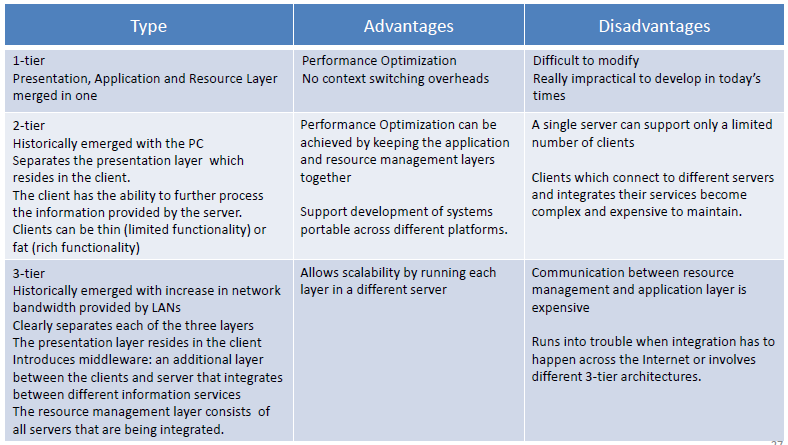
\includegraphics[width=0.64\columnwidth]{layered-archi}
		\end{center}
		\subsubsection{Data abstraction and O-O organisation}
		\begin{itemize}
			\item \textbf{Component}: ADT (Abstract Data Types) or Object that encapsulates data representations and their associated operations e.g. KWIC indexing 
			\item \textbf{Connector}:  Interactions that enable procedure(or method) invocations
			\item \textbf{Pros}: object hides its representation from its clients, allows designers to decompose problems into collections of interacting components
			\item \textbf{Cons}: object must know the identity of the
			other object (not that bad in practice), \textbf{side effects}: if A uses B and C also uses B, then C's
			effects on B can result in unexpected side effects to A,
			and vice versa (unexpected coupling)
		\end{itemize}
		\subsubsection{Shared Repository}
		\begin{itemize}
			\item Maintain all data in a \textbf{central repository} shared by all functional components of a data-driven app. Let the availability, quality, and state of that data \textbf{trigger} and \textbf{coordinate}	the control flow of the application logic (e.g. Repo architecture of IDE)
			\item \textbf{Components}: central data structure that represents current state, collection of independent components that act on central data store
			\item \textbf{Connectors}:Interactions between the repository and the other components
			\item \textbf{Pros}: Independent clients, decouples data storage from manipulation, east to add clients, can share large amount of data
			\item \textbf{Cons}: Communication between clients are slow, subsystems must agree on DB structure
		\end{itemize}
		\begin{center}
			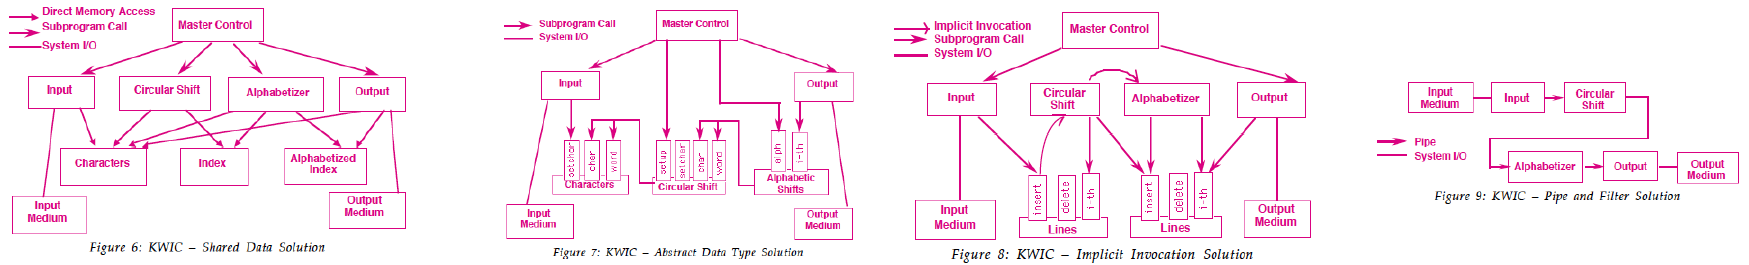
\includegraphics[width=1\columnwidth]{kwic}
		\end{center}
%		\subsection{Decomposition - Guiding Principle}
%		Divide and Conquer, Keep abstraction as high as possible (e.g. don't do into details like what database is used), Increase cohesion, reduce coupling, reuse (design for reuse and reuse design), follow open-close principle to design for flexibility
		\subsection{Types of Cohesion}
		\begin{itemize}
			\item \textbf{Functional} (best, only performs 1 calculation w/o side effects), \textbf{Layer} (related services kept together), \textbf{Communicational} (work on same data), \textbf{Sequential} (work in sequence), \textbf{Procedural} (called 1 after another), \textbf{Temporal} (same phase of execution),
			\textbf{Utility} (weakest, related utilities)
		\end{itemize}
%		\begin{tabular}{|p{0.2\linewidth} | p{0.65\linewidth}|}
%			\hline
%			Type  & Comment \\ \hline
%			Functional & Facilities perform only one computation with no side effects \\ \hline
%			Layer & Related services are kept together, everything else is kept out, and	there is a strict hierarchy in which higher-level services can access	only lower-level services. Accessing a service may result in side effects \\ \hline
%			Communicational & Facilities for operating on the same data are kept together \\ \hline
%			Sequential & A set of procedures, which work in sequence to perform some computation, are kept together. Output from one is input to the next \\ \hline
%			Procedural & A set of procedures, which are called one after another, are kept together \\ \hline
%			Temporal & Procedures used in the same general phase of execution, such as initialization or termination, are kept together \\ \hline
%			Utility & Related utilities are kept together, when there is no way to group them using a stronger form of cohesion \\ \hline
%		\end{tabular}
		\subsection{Types of Coupling}
		\begin{tabular}{|p{0.2\linewidth} | p{0.65\linewidth}|}
			\hline
			Type  & Comment \\ \hline
			Content (tightest) & Component modifies internal data of another \\ \hline
			Common/global & Modules using shared DB or same global variable \\ \hline
			Control & One module (A) directly controls the other (B) by passing information
			on what B should do; \\ \hline
			Data & One module sharing data with another module; e.g., via	passing parameters \\ \hline
			External & A dependency exists to elements outside the scope of the	system, such as the operating system/shared libraries/hardware \\ \hline
			Temporal & Two actions are bundled together just because they happen to occur at the same time \\ \hline
			Inclusion/import (weakest) & Including a tile or importing a package \\ \hline
		\end{tabular}
		\subsection{Architecture Diagrams}
		\begin{itemize}
			\item Shows the "big picture" of what is being built, a shared vision of the dev team, used as a "map" to navigate source code, useful for onbaording new devs to the team.
			\item \textbf{Common mistakes}: notation (colors, shapes) is inconsistent or not explained, purpose and meaning of element is ambiguous, relationship are missing, generic terms used, technology choices omitted, levels of abstraction mixed, too much/too little detail, no logical starting point
			\item "Software System" is the highest level of abstraction and represents something that delivers values to users.
			\item "Container" is a context or boundary inside which code is executed / data stored. Should be separately deployable
			\item "Component" groups related functionality and are not separately deployable units. All components inside a container typically execute in same process space. e.g. JAR files, DLL, shared lib
		\end{itemize}
		\section{MV* Architecture}
		\subsection{MVC}
		\begin{itemize}
			\item Split up into \textbf{View} (GUI/CLI or any output), \textbf{Controller} (acts as mediator, controls what view can show) and \textbf{Model} (Persistence + Business Logic, typically most independent)
			\item View and controllers can be played by same object when it's very tightly coupled
			\item Variant where input goes through view is common (e.g. filling up a form)
			\item Controller acts as listener (to user request and propagate to model), View acts as observer and Model acts as observable
			\item Benefit of \textbf{Separation of Concern} (modularity, output separated from input handling, output and input separated from application state (model) and transaction processing) and \textbf{facilitating extensibility} (multiple views can be created from same model, new functionality can be added to the model independently of other components)
		\end{itemize}
		\subsection{MVA (Model-View-Adapter) / Mediated MVC}
		\begin{itemize}
			\item All communication between Model and View flows through Controller (\textbf{completely decouples view and model}), Controller (adapters/mediators) becomes communication hub
			\item Possible to have \textcolor{red}{different adapters} doing different business logic
		\end{itemize}
		\subsection{MVP (Model-View-Presenter)}
		\begin{itemize}
			\item Popular in .NET world where \textbf{Model} represents business entities/domain models/object model of business tier, \textbf{View} is a lightweight UI only component who isn't aware of the model and \textbf{Presenter} presents user actions to backend system and response to user
			\item View could be further divided in to \textbf{Passive View} (view doesn't know model) and \textbf{Active View} (data binding or simple code in view). Only has \textcolor{red}{1 presenter}
		\end{itemize}
		\subsection{Presentation Model (PM) and Model-View-View-Model (MVVM)}
		\begin{itemize}
			\item PM is well suited for rich UI application / advances in UI technologies
			\item View elements are directly bound to properties on the model ("1-to-1" binding between view and model)
			\item \textbf{Model} represents the state of the view and might contain UI elements specific properties which will be rendered once model is constructed. \textbf{View} is lightweight and simple and is used to publish events raised by user to Presentation Model. \textbf{Presenter} receives event from view, updates the model and any state changes and call the view to render
			\item MVVM is very similar to PM except that it substitutes Presenter with a View-Model. Used in cases like live word count updates, loading screens and validation of form fields
			\item MVVM uses commands and data binding to communicate
		\end{itemize}
		\subsection{Web MVC}
		\begin{itemize}
			\item Very similar to normal MVC except that the controller has a new responsibility of handling the initial HTTP request. Used by frameworks like Spring, Ruby on Rails, PHP, ASP.net
			\item Controller does not do much computation and just serves HTML pages, View could use data from Model to generate static pages, browser only renders what View sends it
			\item New \textbf{Single Page Application} Paradigm introduced an extra step in creating static bundles of HTML, JS and CSS for direct hosting via a \textbf{View Controller}. SPA applications could have the entire MVC in the browser and include logic for making HTTP API requests to API controllers who responds in JSON format
		\end{itemize}
		\begin{center}
			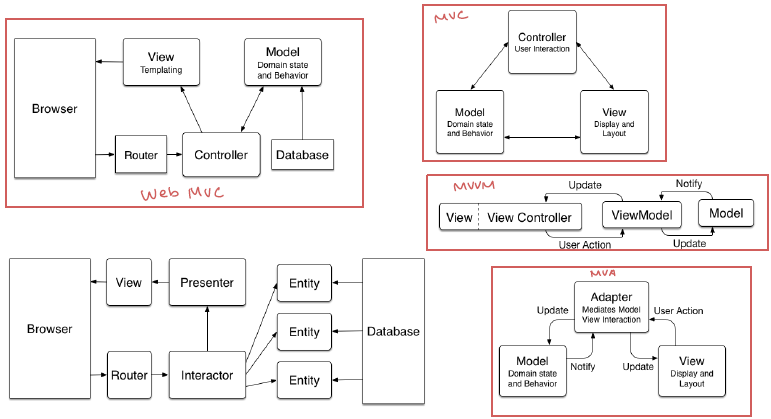
\includegraphics[width=0.6\columnwidth]{MV-star}
		\end{center}
		\subsection{nginx case study}
		\begin{itemize}
			\item nginx has NFRs in Performance, Load (density) and Economic resource utilization. It use a Modular, event-driven, asynchronous (want to waste less time and resource busy waiting), single-threaded,
			non-blocking architecture
			\begin{itemize}
				\item Uses multiplexing (packing multiple request into 1) and event notifications and dedicates specific tasks to separate processes
			\end{itemize}
		\item Workers accepts new requests via shared "listen" (all HTTP requests captured by listener), run-loop relies on async task handling implemented through modularity, event notifications and extensive use of callback functions. Aims to be \textbf{as non-blocking as possible} (can't be completely non-blocking due to disk I/O when disk is filled)
		\item No process/thread per connection (unlike web servers) which makes memory usage very conservative and efficient. Also no create-destroy cycle which save CPU cycles
		\item High scalability due to horizontal scaling on workers to handle more connections $\rightarrow$ scales across multiple cores
		\item Efficient due to caching (reduce I/O ops) in the form of hierarchical data storage on file system and is a shared memory accessed by worker, cache loader and manager
		\end{itemize}
		\subsection{Twitter AdServer Case Study}
		\begin{itemize}
			\item Key considerations: build quickly, iterate frequently, profit oriented
			\item Started off with monolithic as they wanted reliability, deployability and performance and wanted a Cohesive Monolithic Adserver (AdMixer + AdShart)
			\item Faced problems when they wanted to extend to other forms of ads (needed to replicate AdServer for each type of ad which is an Anti-Pattern since each vertical lacks cohesion and there is no reusability). Had troubles reusing existing patterns in legacy code and needed patchy updates. Also had tightly coupled codebase which increased complexity and had spaghetti code
			\item Moved towards microservices by identifying "tech functions" like Candidate Selection, Candidate Ranking and Analytics
			\item Horizontal components are now shared across verticals which led to more cohesive services, decoupling and isolation of verticals and had better separation of concerns
			\item Horizontal services now each serve different kind of ads and it is easily extensible which led to faster development, troubleshooting and debugging
			\item Downside of microservice was that it increased hardware and operational costs and had to redesign the entire system which took time. 
		\end{itemize}
		\section{Microservices}
		\subsection{Modularization}
		\begin{itemize}
			\item \textbf{Module}: deployable (if it's a library), manageable, unit of software that provides a concise interface to its clients (does not expose its internals)
			\begin{itemize}
				\item Code that does not expose its API i.e. Dead code, should not be a module!
			\end{itemize}
			\item Modularization is the process of \textbf{separating the  functionality} of a program into independent modules, such that each contains everything necessary to \textbf{execute only one aspect of the desired functionality}
		\end{itemize}
		\subsubsection{Modular Application}
		\begin{itemize}
			\item \textbf{Monolith}: single application deployed as a single process
			\item \textbf{Modular Monolith}: Monolith composed of loosely coupled, highly cohesive modules 
			\item Splitting application into independent modules allows for \textbf{easier development, better testability and maintainability} and \textbf{allows for reusability} (requires experience to know what can be reused)
		\end{itemize}
		\subsubsection{High Cohesion, Loose Coupling}
		\begin{itemize}
			\item loosely coupled module \textbf{knows as little as it needs to} about the modules with which it interacts
			\begin{itemize}
				\item want to limit number of different types of calls between modules $\rightarrow$ chatty communication leads to performance issues and tight coupling
			\end{itemize}
			\item want \textbf{related behaviors to be grouped together} and unrelated behavior elsewhere $\rightarrow$ leads to high cohesion
			\item want to find \textbf{boundaries} to ensure related stuff are in 1 module and communicates with other modules as loosely as possible
		\end{itemize}
		\subsubsection{Design Principles}
		\begin{minipage}{0.6\columnwidth}
			\begin{center}
				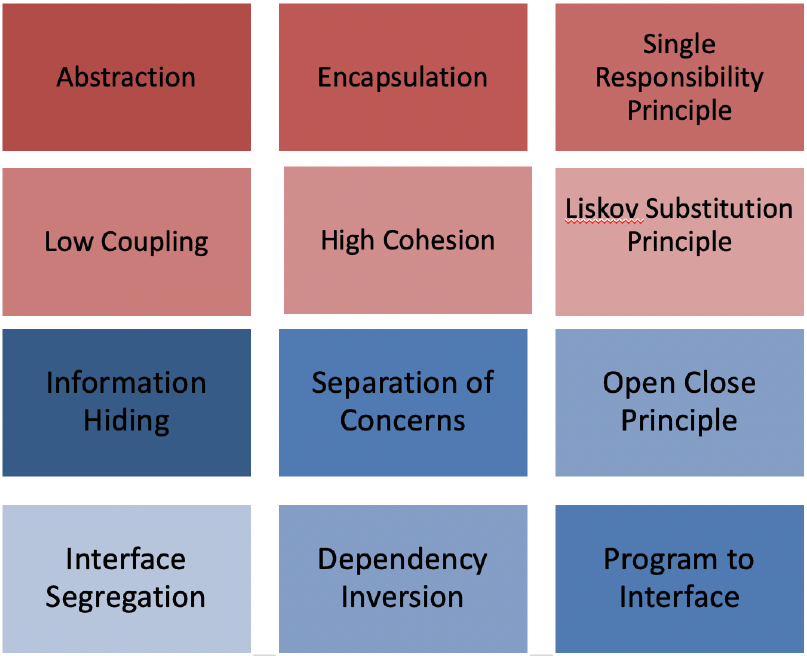
\includegraphics[width=0.65\columnwidth]{design-principles}
			\end{center}
		\end{minipage}
		\begin{minipage}{0.4\columnwidth}
			\begin{itemize}
				\item \textbf{Information Hiding}: Guides you on how to define boundaries
				\item want to separate code that change frequently from static code
				\item Hide code that changes so that we can make changes internally without affecting compatibility
				\item \textbf{Encapsulation}: binding one or more things into 1 boundary
				\item Use visibility to hide parts of implementation
			\end{itemize}
		\end{minipage}
		\subsection{Command-Query-Responsibility Segregation (CQRS)}
		\begin{itemize}
			\item \textbf{pattern} relying on separation of \textbf{commands} (writes) from \textbf{queries} (reads)
			\item \textbf{Command}: operations that change application state but returns no data, will leave side effect within application
			\item \textbf{Queries}: return data but don't change application state
			\item Models for read operations and write operations are \textbf{completely separated} (could be using 2 different tables for SQL DB or could use 2 entirely different DB e.g. SQL and NoSQL) $\rightarrow$ allows for \textbf{individual scaling/caching of reads/writes}
			\item \textbf{Command model will go through the domain model} since it is modifying the state (may require some manipulation of data and it requires the entire transactional entity) but Query model can \textbf{go directly to persistence layer} to fetch data 
			\item If implemented using 2 different data stores, will \textbf{require some sort of synchronization} between write store and read store so that when you read data it is updated
			\item Follows the \textbf{Separation of Concern}, \textbf{Single Responsibility} and \textbf{Interface Segregation}
			\begin{itemize}
				\item responsibility of handling writes separated from reads
				\item Each model does one thing only, either read or write
				\item Client either talks to read or write interface
			\end{itemize}
		\end{itemize}
		\subsection{Emergence of Microservices}
		\begin{itemize}
			\item Defined as an \textbf{\textit{independent, standalone capability}} designed as an executable that \textbf{\textit{communicates with other microservices}} through standard lightweight inter-process communication such as HTTP, message queues, etc.
		\end{itemize}
		\begin{tabular}{l l}
			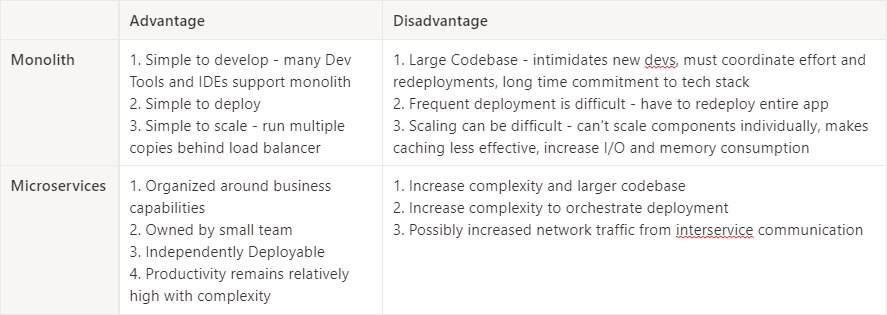
\includegraphics[width=0.47\columnwidth]{monolith-vs-microservices}
			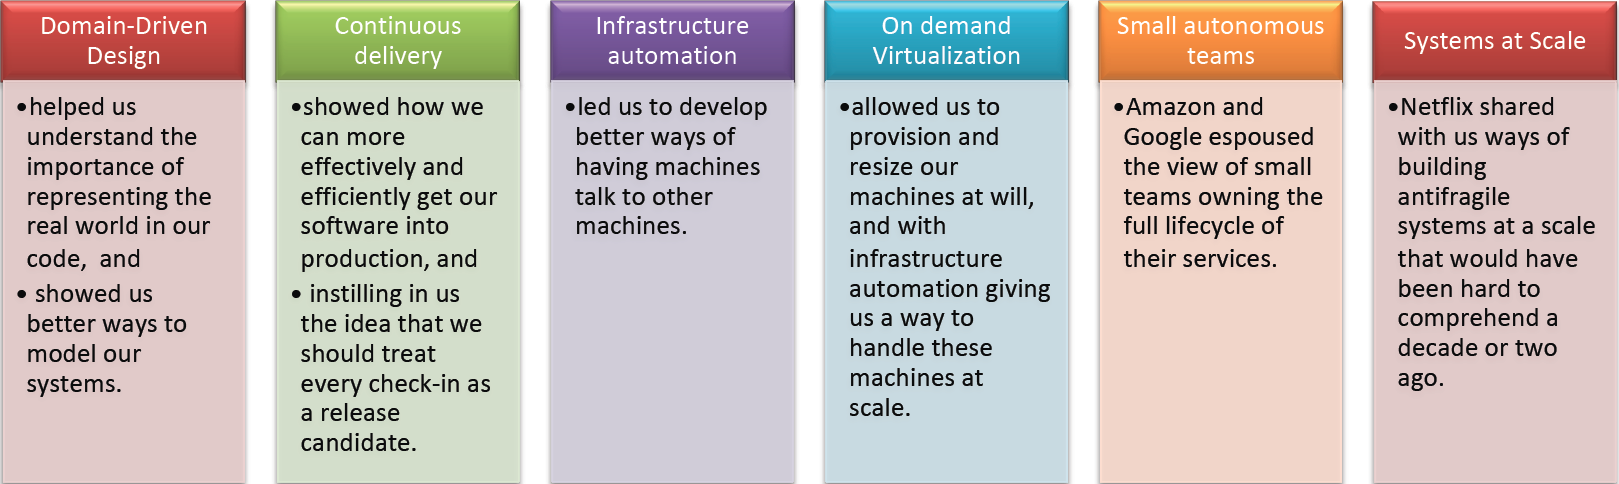
\includegraphics[width=0.54\columnwidth]{microservices-emergence}
		\end{tabular}
		\subsection{Characteristics of Microservices}
		\subsubsection{Domain Driven Design (DDD)}
		\begin{itemize}
			\item DDD does not dictate any specific architecture style, only \textbf{requires model to be isolated from technical complexities} so that it can\textbf{ focus on domain logic concerns}
			\item \textbf{Domain}: critical and fundamental /foundational concept behind the business
			\item \textbf{Ubiquitous Language}: A shared language between domain experts and developers that uses domain-specific terminology
			\item \textbf{Subdomain}: is a logical "separation" of the domain, is in the \textcolor{red}{problem space}
			\begin{itemize}
				\item \textbf{Core} - "must have functions", key differentiator of the business
				\item \textbf{Supporting} - "nice to haves", related to business but not differentiator, outsources or implemented in-house
				\item \textbf{Generic} - not specific to business, typically outsourced
			\end{itemize}
			\item \textbf{Bounded Context}: Divide complex and large domain into separate bounded context which is a explicit boundary within which a domain model exists
			\begin{itemize}
				\item Bounded context refers to the \textcolor{red}{solution space} $\rightarrow$ solves problem from sub-domain
				\item 1 bounded-context can contain \textbf{multiple sub-domains} and is the \textbf{actual implementation of sub-domains}
				\item Inside the boundary, \textbf{all terms and phrases of the ubiquitous language have specific meaning} $\rightarrow$ customer in a Sales Context can mean something different from a customer in the Support Context
				\item Follows \textbf{SoC} and \textbf{SRP} as each part of the system has its own intelligence, data and vocabulary and is independent of each other
			\end{itemize}
		\end{itemize}
		\subsubsection{Microservices}
		\begin{itemize}
			\item \textbf{verb/use cases} responsible for particular actions
			\item \textbf{nouns/resources} responsible for operations on entities/resources of given type
			\item Use \textbf{subdomains} that corresponds to different parts of the business 
			\item Use\textbf{ Bounded context} that have \textbf{physical boundaries} and are \textbf{owned by a single team}
			\begin{itemize}
				\item One team can own multiple microservices
				\item \textcolor{red}{Microservices are bounded context but all bounded contexts are not microservices} $\rightarrow$ bounded contexts sometimes have wide functionalities
			\end{itemize}
			\item Each service should \textbf{ideally only have small set of responsibilities} $\rightarrow$ apply SRP
			\item Aim to target services that encompasses entire Bounded Context
		\end{itemize}
		\subsubsection{Characteristics of Microservices}
		\begin{enumerate}
			\item Organized around business capabilities
			\begin{itemize}
				\item Looks at what functionality does it provide and what data does it need?
			\end{itemize}
			\item Loosely coupled
			\begin{itemize}
				\item \textbf{Aggregates}: a \textbf{self-contained unit focused on a single domain} concept in the system
				\item \textbf{Bounded contexts}: represents a \textbf{collection of aggregates}, with an explicit interface
				\item Use \textbf{information hiding}  and \textbf{async communication} when possible!!
				\begin{itemize}
					\item \textbf{Inside-out thinking} - Specify an API for external services to interact
					\item \textbf{Outside-in thinking} - External service specifies an interface for internal service to implement
				\end{itemize}
			\end{itemize}
			\item Owned by small (cross-functional) team
			\begin{itemize}
				\item When teams are less coupled, product also tend to be less coupled (Conway's Law)
			\end{itemize}
			\item Independently deployable
			\begin{itemize}
				\item Each microservice has its own deployment, resource, scaling and monitoring requirements
				\item \textbf{Service per Host} (e.g. EC2) VS \textbf{Service per Container} (e.g. Docker)
			\end{itemize}
		\end{enumerate}
		\subsubsection{Services and their Database}
		\begin{itemize}
			\item \textbf{Database per service pattern}: Each service has its \textbf{own database schema} which often leads to data duplication but is however needed for loose coupling. Can choose database suited for service
		\end{itemize}
		\subsubsection{Service Communication}
		\begin{itemize}
			\item Inter process communication can either be async or sync
			\begin{itemize}
				\item \textbf{Request/sync response} - client makes request to service and waits for response
				\item  \textbf{Notification} (one way request) - client sends request to service but no reply is expected
				\item \textbf{Request/ Async response} - client sends request to service which replies asynchronously
			\end{itemize}
		\end{itemize}
		\subsubsection{API Gateway}
		\begin{itemize}
			\item API Gateway acts as a server that is the \textbf{single entry point} into the system 
			\item It encapsulates the internal system architecture and provides an API tailored to each client $\rightarrow$ client does not have to directly communicate to the services and offloads routing workload to API gateway
			\item Could have other responsibilities like authentication, monitoring, load balancing and caching
			\item Follows the \textbf{facade pattern}!
		\end{itemize}
		\subsubsection{Orchestration vs Choreography}
		\begin{itemize}
			\item \textbf{Orchestration}: rely on a central brain to guide and drive the process
			\begin{itemize}
				\item central brain could be a bottleneck and a single point of failure
			\end{itemize}
			\item \textbf{Choreography}: inform each part of the system of its job, and let it
			work out the details
			\begin{itemize}
				\item more decoupled but more work if monitoring is needed
			\end{itemize}
		\end{itemize}
		\subsubsection{Service Discovery}
		\begin{itemize}
			\item API Gateway needs to know the IP address and port of each microservice
			\item Could either do Client-side Discovery, Server-side Discovery or a Service Registry
			\begin{itemize}
				\item Client-side Discovery: \textbf{Client queries service registry} which maintains a database of services instance (if service terminates than it is removed from registry). Client then determines network location of available service using a load balancer (\textbf{couples client with service registry})
				\item Server-side Discovery: Client \textbf{makes request to service via load balancer} which queries service registry and routes each request to an available service instance (\textbf{decouple client from service registry but require manual implementation of load balancer})
				\item Service registry: is a database of services, their instances and locations, \textbf{requirement of being highly available and up to date}
			\end{itemize}
			\item Allows services to register itself and allows services to be discovered by the registry
		\end{itemize}
		\begin{center}
			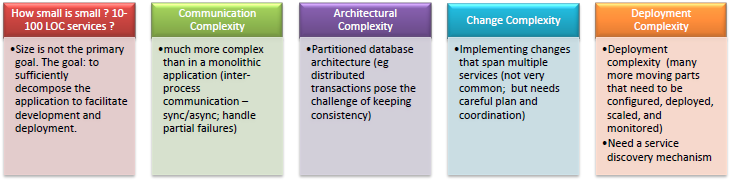
\includegraphics[width=0.75\columnwidth]{microservices-challenges}
		\end{center}
		\section{Messaging Patterns}
		Messaging systems or Message Oriented Middleware (MOM) are pieces of software that provides messaging capabilities. All Distributed Application Design (DAD) needs a MOM.
		\begin{itemize}
			\item 3 axes of component/application communication: \textbf{sync vs async}, \textbf{single vs multiple receiver}, \textbf{persistent vs transient} 
			\item Persistent Async (Email), Persistent Sync (Messaging/Chat), Transient Async (UDP), Transient Sync (RPC), Sync Single (RPC, REST), Async Single (Polling, P2P), Sync Multiple (Webhooks), Async Multiple (PubSub)
		\end{itemize}
		\subsection{Communication Types}
		\subsubsection{Synchronous vs Asynchronous}
		\begin{itemize}
			\item \textbf{Synchronous}: components exchanges information at the same time with each other. a.k.a. "1:1" or "request-reply" communication. 
			\begin{itemize}
				\item Tight coupling, connection overhead, sender has to handle failures
			\end{itemize} 
			\item \textbf{Asynchronous}: communication has lag between message sent and receiver response. Enables independent functioning of receiver and sender and 1:n communication
			\begin{itemize}
				\item Notification need to be sent and sender needs to remember context which message was sent
			\end{itemize}
		\end{itemize}
		\subsubsection{Remote-Procedure Call (RPC)}
		\begin{itemize}
			\item RPC mimics the serial thread of execution that a "normal" non-distributed system would use, each statement is executed in sequence (\textbf{sync} in nature)
			\item \textcolor{red}{Success of one RPC call depends on success of all downstream RPC call} ("all or nothing")
			\item Type of \textbf{inter-process communication} to make a procedure execute on another address space (typically another computer in shared network)
			\item Client call to procedure $\rightarrow$ Stub builds message (Marshalling) $\rightarrow$ Message sent via network $\rightarrow$ Server OS hands stub message to server stub and unpacks it (Un-marshalling) $\rightarrow$ Stub makes local call to method
		\end{itemize}
		\subsubsection{HTTP/HTTPS}
		\begin{itemize}
			\item Is a \textbf{sync request-reply} pattern
			\item In the event that backend processing needs to be asynchronous but requester needs a clear response, one possible way to circumvent it is to keep polling status endpoint
		\end{itemize}
		\subsubsection{Asynchronous Message-passing}
		\textbf{Async and persistent}, with intermediate storage (message queue) while sender and receiver are not active. \textbf{Can be single} (P2P, exactly 1 consumer and message processed once)/\textbf{multiple} (pub-sub) receiver. Messages guaranteed to be inserted into the queue but no guarantee on when or if message will be read.
		\subsubsection{Persistent vs Transient}
		\begin{itemize}
			\item Persistent (store-and-forward): messages stored in intermediate hop, receiver \textbf{guaranteed to receive message}. Has 4 stages - send, received, read, processed (e.g. Emails)
			\item Transient: message buffered \textbf{only for a short period of time} (while sender/receiver are executing). Discarded if cannot be delivered or host is down (e.g. TCP/IP)
		\end{itemize}
		\subsection{Messaging Pattern}
		Messaging systems constructs, transports, routes, transforms, produce and consume messages. Also manage and test the system.
		\subsubsection{Message Construction}
		\begin{itemize}
			\item Each message has a \textbf{header} (metadata), \textbf{properties} (optional) and \textbf{payload} (data).
			\item Encapsulates \textbf{method requests} and \textbf{data structure} to be sent. Header specifies the type of information transmitted, origin, destination, size and other structural information
			\item 3 types of message intent: \textbf{Command message} (telling consumer what to do), \textbf{Document message} (just sending data), \textbf{Event message} (Notification, have time constraint, cannot have too high latency)
		\end{itemize}
		\subsubsection{Message Channel}
		\begin{itemize}
			\item Connect sender and receiver using a \textbf{queue} that allows them to exchange messages
			\item Request/reply channel: channel transmit message in \textbf{1 direction}. If we want two-way message, need a channel for each of reply and request
			\item Contains \textbf{return address} (to tell replier where to send reply to), \textbf{correlation ID} (specifies which request the reply is for. Contains requestor, replier, request, reply, request ID and correlation ID. \textbf{Can be chained} $\rightarrow$ allows for retrace of message from latest reply to original request)
			\item \textbf{Point to Point} (P2P): request processed by single consumer$\rightarrow$ uses message queues
			\item \textbf{Publish-Subscribe}: used when \textbf{multiple parties} are interested in certain messages. Messages published to a topic is \textbf{immediately received} by all subscribers (unless message filter is applied)
			\begin{itemize}
				\item beneficial when it is important to communicate with multiple services that do work in parallel and \textbf{needs responses to be aggregated afterwords}
				\item Has \textbf{Invalid Message channel} (handles message that makes no sense), \textbf{Dead Letter Channel} (handles message that cannot be delivered), \textbf{Data Type Channel} (separate channel for each type of data e.g. XML, JSON, byte array etc.)
			\end{itemize}
		\end{itemize}
		\subsubsection{Message Routing}
		\begin{itemize}
			\item Consumes messages from 1 channel and reinserts them into different channels based on set of conditions
			\item \textbf{Simple router} which route messages from 1 inbound channel to $\geq$ 1 outbound channels. \textbf{Composed Routers} which combines multiple simple router to create complex message flows
			\item \textbf{Content-Based}: Examines message content and
			routes $\rightarrow$ has knowledge of all possible recipients and their capabilities. \textbf{Message filter is a special kind of content-based router} that discards messages based on content. \textbf{Decouples receiver and sender}
			\item \textbf{Context-based}: Decides destination based on context,
			e.g. load-balancing, fail-over
			\item \textbf{Message Splitter}: Splits a single message into multiple messages, \textbf{not a router}
			\item \textbf{Message Aggregator}: Aggregates correlated messages
			into a single message
			\item \textbf{Scatter Gather}: Broadcast to multiple participants
			and aggregates replies into 1 message
		\end{itemize}
		\subsubsection{Message Transformation}
		\begin{itemize}
			\item Transforms application layer data structures/types/representation e.g. ASCII to Unicode, TCP/IP to Sockets etc. so that systems using different data formats can communicate
			\item Uses a \textbf{Message Translator} which is responsible for the conversion between file formats $\rightarrow$ follows a \textbf{Channel Adapter Pattern}
			\item Helps to decouple applications from each other as they do not need to know about each other's data formats
			\item Could also use a \textbf{Canonical Data Model} which provides an additional layer of indirection $\rightarrow$ all data will be first converted to canonical data format, sent, then translated back to its own data format at receiver end
			\item Can contain a \textbf{Message Endpoint} which is an interface between an application and a messaging system $\rightarrow$ should be an isolated piece of code from the rest of the application
			\begin{itemize}
				\item Endpoint can be used to either send/receive message but \textbf{1 instance does not do both}
				\item Endpoint is channel specific $\rightarrow$ multiple endpoints to interface with multiple channels
				\item \textbf{Polling Consumer}: controls when it consumes messages, \textbf{proactively} reads messages. \textbf{Event-Driven Consumer}: message delivery is an event that trigger receiver, \textbf{reactively} process messages
			\end{itemize}
		\end{itemize}
		\section{Design Patterns}
		Design pattern is a \textit{solution} (pattern itself, general design) to a \textit{recurring problem} (goal and constraints to be achieved, aka \textbf{forces}) in a \textit{context} (situation in which pattern applies). A pattern consists of a name, classification, intent (what the pattern does), participants (responsibilities of classes/objects involved), Implementation/Sample Code.
		\subsection{GoF Patterns Category}
		\begin{itemize}
			\item \textbf{Creational Patterns} - help designers handle issues with creation of objects, \textbf{encapsulate/hide details} about actual creation
			\item \textbf{Structural Pattern} - provide structure to relationship between objects, allows for \textbf{flexibility} in interconnecting modules
			\item \textbf{Behavioral Patterns} - help define how objects talk with each other, \textbf{increases communication flexibility}, \textbf{simplify flow} and \textbf{make communications more understandable}
		\end{itemize}
		\subsubsection{Principles of GoF}
		\begin{itemize}
			\item \textbf{Program to interface/abstract class} - want to depend on interfaces only so that we are decoupled from implementation $\rightarrow$ implementation can vary without affecting application, \textbf{healthy dependency relationship}
			\item Favor Composition/aggregation over inheritance (\textbf{has-a over is-a}) - Inheritance causes tight coupling between base class and subclass $\rightarrow$ use composition to reduce coupling
			\item \textbf{Encapsulate what 'varies'} - separate code that varies from code that does not vary (static code) so that we can alter the part that varies without affecting the static code
		\end{itemize}
		\subsection{Creational Pattern}
		\subsubsection{Builder}
		\begin{itemize}
			\item useful for objects with many possible constructor parameters
			\item \textbf{Intent}: Separate the construction of a complex object from its	representation so that the same construction process can create different representations $\rightarrow$ client separated from object creation process
			\item Enforces \textbf{step-by-step process} which remains the same but end products can be different
			\item \textbf{Participants}: \textbf{Product} (class that represent product to be created), \textbf{Director} (class that dirrects \texttt{Builder} to perform steps), \textbf{Builder} (interface to build parts), ConcreteBuilder (class that implements Builder)
		\end{itemize}
		\subsubsection{Prototype}
		\begin{itemize}
			\item used in cases when a specific resource is expensive to create (e.g. need to call outside API)
			\item \textbf{Intent}: create an object by cloning another as necessary 
			\item Client does not instantiate a product directly,  calls the \texttt{clone()} method of the prototype
			\item \textbf{Participants}: \textbf{Client}, \textbf{Prototype} (interface or abstract class that defined contract of classes that permits cloning), \textbf{ConcretePrototype} (class that provides cloning operations)
		\end{itemize}
		\subsection{Structural Patterns}
		\subsubsection{Adapter (aka Wrapper)}
		\begin{itemize}
			\item allows interface of existing class to be used from another interface, follows \textbf{SRP} and \textbf{dependency inversion principles}
			\item \textbf{Intent}: convert interface into something that is compatible with what the client expects
			\item \textbf{Participants}: \textbf{Client}, \textbf{Target} (existing interface client communicates with), \textbf{Adaptee} (new incompatible interface), \textbf{Adapter} (class that adapts adaptee to target)
		\end{itemize}
		\subsubsection{Facade}
		\begin{itemize}
			\item \textbf{Intent}: provide unified interface to a set of interfaces in subsystem to make subsystem easier to use
			\item \textbf{internal subsystems still talk to each other} but client just talks with Facade
			\item \textbf{Participants}: \textbf{Client}, \textbf{Facade} (delegates client requests to appropriate subsystem), \textbf{Subsystems} (used by facade but not the other way round, subsystems no reference to facade)
		\end{itemize}
		\subsection{Behavioral Pattern}
		\subsubsection{Observer Pattern} 
		\begin{itemize}
			\item \textbf{Intent}: Let objects observe behavior of other objects so they stay in sync, abstraction has 2 aspect (one dependent on another), change to 1 aspect requires notifying dependents
			\item \textbf{Participants}: \textbf{Subject} (interface/abstract class defining operations for attaching/removing observers), \textbf{ConcreteSubject} (maintain state of object and notify observers when change detected), \textbf{Observer} (interface/abstract class, defines operations to be used to notify this object), \textbf{ConcreteObserver}
			\item Typically used in GUI apps where different views can be rendered for same subject
			\item \textbf{Pull-Model}: register with subject $\rightarrow$ subject change states $\rightarrow$ notify observers $\rightarrow$ \textcolor{red}{observer pull changed data}
			\item \textbf{Push-Model}: mechanism similar to Pull-Model except subject will just push a snapshot of its state to observers instead of notifying them when state changes i.e. \textcolor{red}{observers don't have to manually pull data}
			\item Follows \textbf{OCP}
		\end{itemize}
		\subsubsection{Mediator}
		\begin{itemize}
			\item \textbf{Intent}: Mediator encapsulates how a set of objects communicates which reduces coupling between objects. Objects delegate routing data, messages, request through mediator
			\item \textcolor{red}{Subsystem don't talk to each other} but instead talk to mediator (different from Facade)
			\item \textbf{Participants}: \textbf{MediatorBase} (abstract class that defines communication with Colleague objects), \textbf{ConcreteMediator} (implements Mediator, holds reference to Colleagues it serves), \textbf{ColleagueBase}(abstract class, holds reference to mediator), \textbf{ConcreteColleague}
		\end{itemize}
		\subsubsection{Memento}
		\begin{itemize}
			\item \textbf{Intent}: w/o violating encapsulation, allow client to capture an
			object’s state, and restore
			\item Allows an \textbf{\texttt{Originator}} that can create or restore
			from a \textbf{\texttt{Memento}}, which captures the former’s state.
			A \textbf{\texttt{Caretaker}} can help to safekeep \textbf{\texttt{Mementos}} and clean them
			up when the \textbf{\texttt{Originator}} is deallocated.
		\end{itemize}
		\subsubsection{State}
		\begin{itemize}
			\item \textbf{Intent}: allow an object to alter its behavior when internal state
			changes
			\item Prevent massive switch cases by defining a
			class for each \textbf{\texttt{State}}, and delegating \textbf{\texttt{Context}} behavior
			to those \textbf{\texttt{ConcreteState}} (using polymorphism). Difference with Strategy is that
			\textbf{\texttt{ConcreteStates}} are \textcolor{red}{aware of each other} and transition the
			\textbf{\texttt{Context}}’s \textbf{\texttt{State}} accordingly
			\item Follows \textbf{open-close principle}
		\end{itemize}
		\subsubsection{Strategy}
		\begin{itemize}
			\item \textbf{Intent}: represent a behavior that parameterizes an algorithm for behavior or performance  
			\item Encapsulate algorithms into \textbf{\texttt{Strategy}}, then
			have the \textbf{\texttt{Context}} use the correct \textbf{\texttt{ConcreteStrategy}}. Follows \textbf{open-close principle}
		\end{itemize}
		\subsection{Other Patterns}
		\subsubsection{Data Transfer Object}
		\begin{itemize}
			\item Bundle all data items that might be needed into a single DTO used for querying or updating attributes together. Reduce multiple remote calls into a single call which in turns reduces network traffic. DTO is generally \textbf{immutable and read-only}
		\end{itemize}
		\section{Software Design Quality}
		\begin{center}
			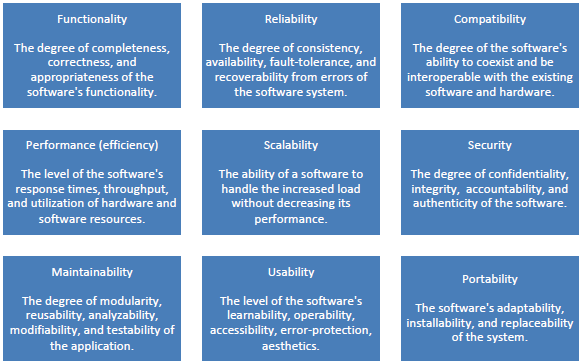
\includegraphics[width=0.64\columnwidth]{quality_attribute}
		\end{center}
		\begin{itemize}
			\item \textbf{Quality Perspective} refers to how good is software design in terms of product and process perspectives
			\item \textbf{Erosion}: overall deterioration of the	engineering quality of a software system that could lead to technical debt
			\item Symptoms of erosion: \textbf{Rigidity} (every change forces many other changes, system hard to change), \textbf{Immobility} (hard to modularize system), \textbf{Fragility} (system break in conceptually unrelated places), \textbf{Viscosity} (doing things correctly is harder), \textbf{Opacity} (code is hard to read and understand)
			\item \textbf{Quality Assurance} follows preventive approach and ensures quality in SE \textbf{processes}. \textbf{Quality Control} is post-development focused, ensuring quality in the review/testing phase
		\end{itemize}
	\end{multicols*}
\end{document}
